\section{ELEC-VQA Dataset Construction}\label{sec:dataset}
\subsection{Sources, Scope, and Sampling Units}
The ELEC-VQA dataset contains 10,201 QA records from 44 DWGs in 14 substation projects. Its 1,019 image configurations comprise 300 original local context windows and 719 controlled native-DWG variants. Original windows include surrounding schematic context and can overlap within a source drawing. Each record retains project, drawing, parent-window, and image-configuration identities, allowing dependent observations to be grouped during partitioning and analysis.

The intended unit of model input is a readable local schematic, rather than a complete drawing sheet. Selection favors windows whose visible external wiring and explicit contact pairs admit a bounded representation. Questions are not restricted to label transcription, but symbol and label recognition remain prerequisites for higher-level tasks. Figure~\ref{fig:pipeline} shows the construction overview, and Table~\ref{tab:splits} reports the partition summary.

\begin{figure*}[t]
\centering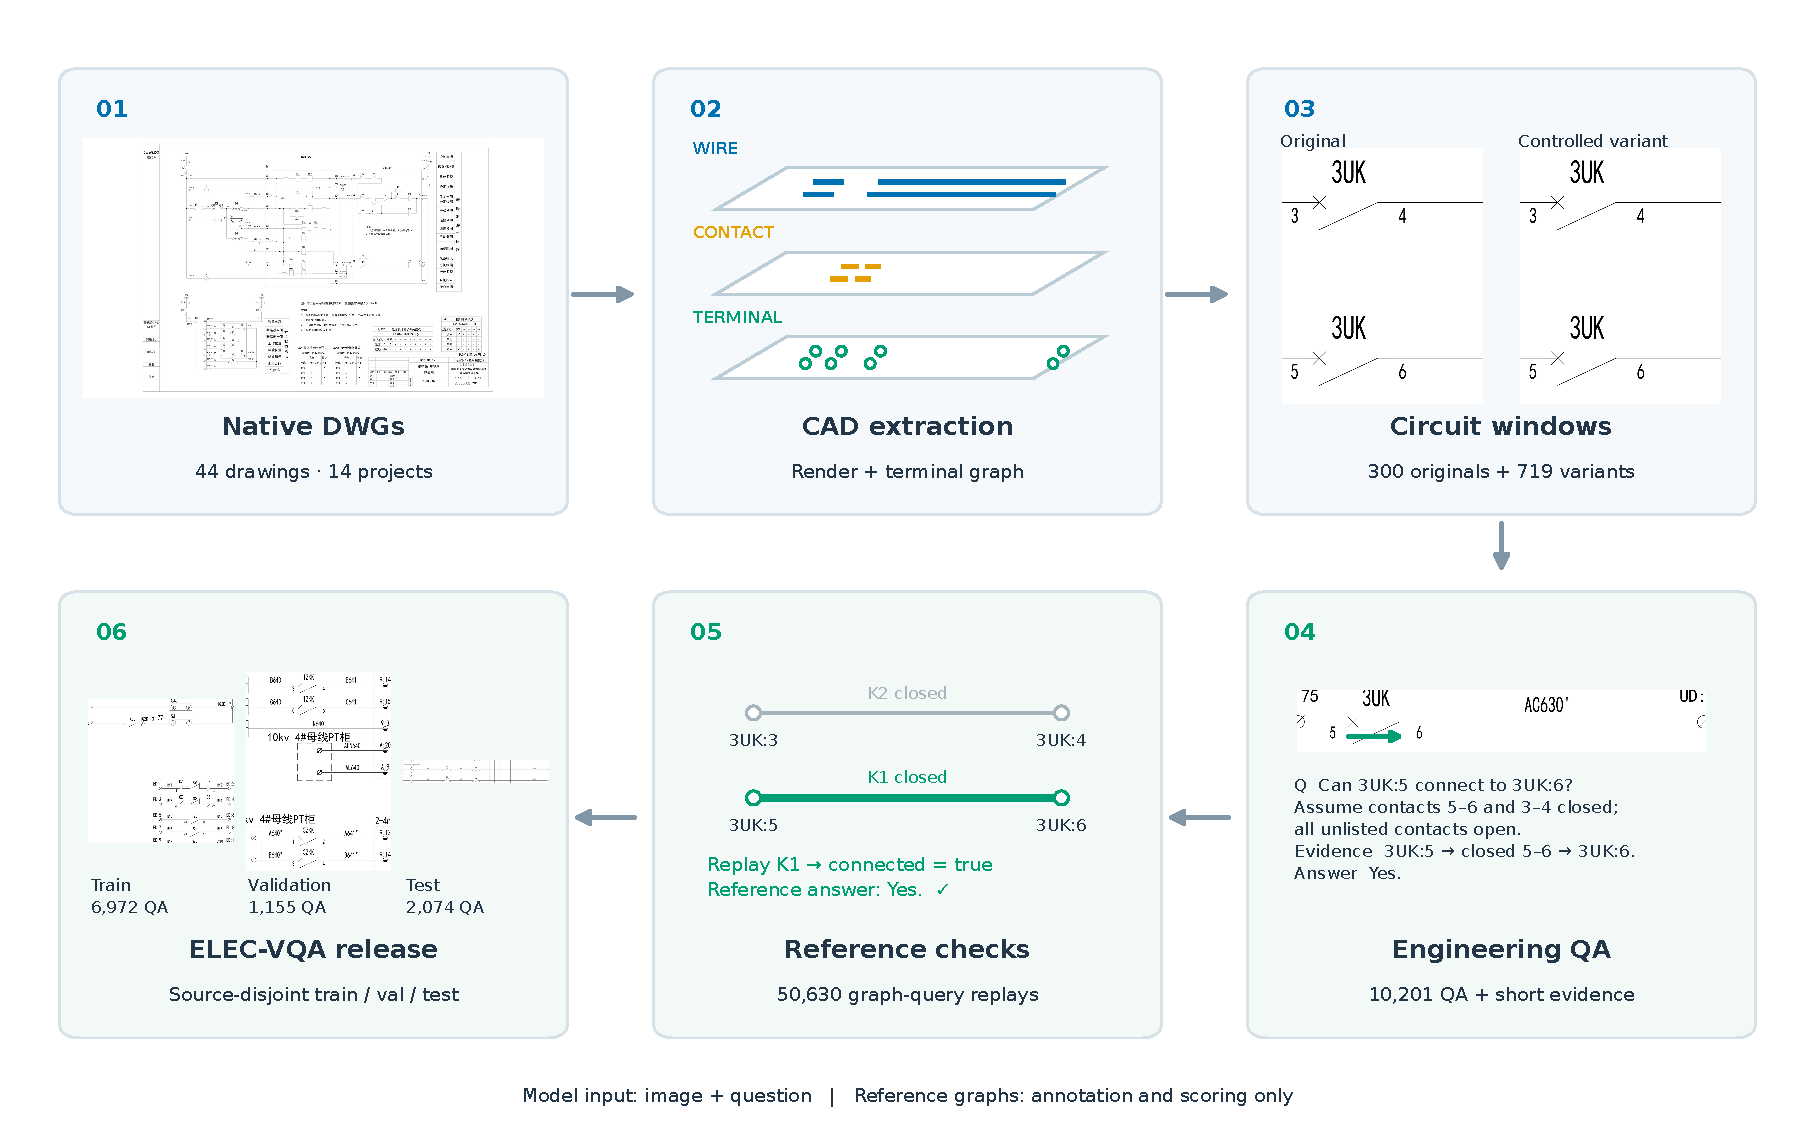
\includegraphics[width=\textwidth]{assets/figure_02.pdf}
\caption{Source-traceable dataset construction. The model receives an image and a question; source graphs and verification queries remain annotation-side information. }
\label{fig:pipeline}
\end{figure*}

\begin{table}[t]
\centering\small\setlength{\tabcolsep}{3pt}
\caption{Source-disjoint partitions. Windows count original contexts; variants count controlled native edits.}
\label{tab:splits}
\begin{tabular}{@{}lrrrrrr@{}}\toprule
Split & Proj. & DWGs & Windows & Variants & Images & QA \\\midrule
Train & 11 & 29 & 218 & 479 & 697 & 6,972 \\
Validation & 1 & 8 & 34 & 88 & 122 & 1,155 \\
Test & 2 & 7 & 48 & 152 & 200 & 2,074 \\
\midrule
Total & 14 & 44 & 300 & 719 & 1,019 & 10,201 \\
\bottomrule\end{tabular}
\end{table}

\subsection{Native Rendering and Source Traceability}
Extraction and rendering use the AutoCAD ActiveX COM interface. Rendering adjusts lineweight while preserving conductor geometry. Geometry entities are assigned a 0.35-mm lineweight without changing their coordinates. Rendering uses font-repaired companion working copies and project-specific plotting settings to produce native vector PDFs, which are rasterized and cropped using the recorded CAD-to-image mapping. This is distinct from raster dilation or generative redrawing. Lineweight adjustment is restricted to rendering; conductor coordinates and junction topology are preserved.

Terminal positions, conductor geometry, source identifiers, crop bounds, and image hashes support traceability. Controlled faults are applied in native working copies and rendered under registered views. Figure~\ref{fig:visual} shows registered crops from an original window and a controlled cross-network link, with their reference graphs. Display crops are distinguished from the full released images supplied to models.

\begin{figure*}[t]
\centering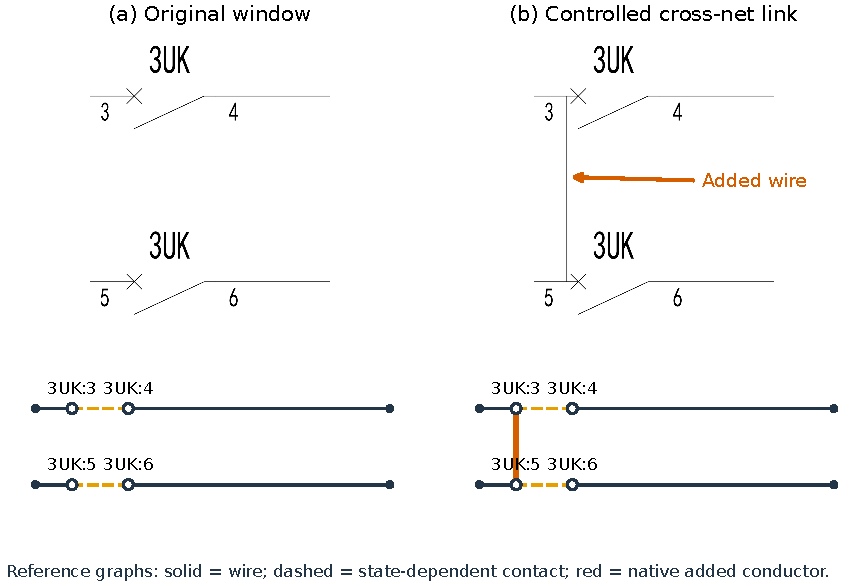
\includegraphics[width=.96\textwidth]{assets/figure_03.pdf}
\caption{Original local window and controlled native-DWG cross-network link. Registered crops show the added conductor connecting 3UK:3 and 3UK:5; the bottom panels show the corresponding bounded reference graphs. Dashed graph edges denote modeled contacts whose states are given by the question. Cropping and the arrow are for display only; models use the full released images.}
\label{fig:visual}
\end{figure*}

\subsection{State-Dependent Electrical Representation}
A local circuit is represented as $G=(V,E_w,E_c)$, where $V$ contains terminals and junctions, $E_w$ contains external conductors, and $E_c$ contains explicitly modeled contact pairs. For a state assignment $s$, removed-wire set $R$, and optional jumper set $J$, the active graph is
\begin{equation}
G_{s,R,J}=\left(V,(E_w\setminus R)\cup\{e\in E_c:s(e)=1\}\cup J\right).
\label{eq:active}
\end{equation}
Reachability in this graph determines bounded continuity. A contact's drawn appearance is not substituted for the state stipulated in the question. For a relevant unknown state, admissible assignments are evaluated separately; the answer may depend on that state. A graphical crossing is not automatically a junction, and undocumented device internals are excluded.

The representation does not establish actual voltage, current magnitude, protection operation, or system safety. Diagnosis assumes the stated fault family, and continuity measurements refer to isolated circuits with intact wires unless otherwise specified. These restrictions make the answer checkable; they also delimit the engineering claim.

\subsection{Questions, Answers, and Compact Evidence}
Fifteen task families cover conditional connectivity (T01), minimum closure (T02), wire groups (T03), contact-opening effects (T04), unknown states (T05), bypasses (T06), fault candidates (T07), measurement selection (T08), stated design requirements (T09), repair checks (T10), path order (T11), contact-network relationships (T12), diagnostic sufficiency (T13), voltage-information sufficiency (T14), and branch interruption (T15). Table~\ref{tab:tasks} reports their distribution. This is a task taxonomy, not fifteen independently validated levels of difficulty.

\begin{table}[t]
\centering\small\setlength{\tabcolsep}{3pt}
\caption{QA counts by task and split. T14 is a diagnostic control, and T12 contains no verified parallel cases.}
\label{tab:tasks}
\begin{tabularx}{\linewidth}{@{}lXrrrr@{}}\toprule
ID & Task family & Train & Val. & Test & Total \\\midrule
T01 & Connectivity & 1,495 & 259 & 440 & 2,194 \\
T02 & Minimum closure & 666 & 103 & 181 & 950 \\
T03 & Wire groups & 697 & 122 & 200 & 1,019 \\
T04 & Opening effects & 665 & 103 & 181 & 949 \\
T05 & Unknown states & 665 & 103 & 181 & 949 \\
T06 & Bypass analysis & 665 & 103 & 181 & 949 \\
T07 & Fault candidates & 471 & 58 & 127 & 656 \\
T08 & Measurement plan & 467 & 58 & 127 & 652 \\
T09 & Requirements & 697 & 122 & 200 & 1,019 \\
T10 & Repair checks & 130 & 24 & 69 & 223 \\
T11 & Path order & 164 & 30 & 57 & 251 \\
T12 & Contact relations & 60 & 20 & 40 & 120 \\
T13 & Diagnosis sufficiency & 60 & 20 & 40 & 120 \\
T14 & Voltage sufficiency & 10 & 10 & 10 & 30 \\
T15 & Branch interruption & 60 & 20 & 40 & 120 \\
\midrule Total & & 6,972 & 1,155 & 2,074 & 10,201 \\
\bottomrule\end{tabularx}
\end{table}

Questions use circuit-aware templates and controlled wording variants. Their language is English except where a source annotation must be quoted. A single image supports different decisions rather than repeated paraphrases counted as new semantic cases. Each master record separates the short answer, typed result, compact evidence steps, source entities, and verification queries. The evidence states the relevant condition, a conducting route or blocking fact, and only the alternatives necessary to justify the conclusion. Paths are certificates for positive reachability; negative statements retain the solver's reachable region in the structured record rather than claiming that an omitted route proves disconnection.

Evidence text is limited to 192 tokens under the local Qwen tokenizer, excluding headings and the answer; the published maximum is 189 and the mean is 39.63. Over-budget candidates are excluded rather than truncated. Figure~\ref{fig:distribution} shows the task, evidence-length, and image-provenance distributions. T12 currently contains series and separate-network cases but no verified parallel examples. T14 contains only negative sufficiency answers and is treated as a diagnostic control, not evidence of learned visual reasoning.

\begin{figure*}[t]
\centering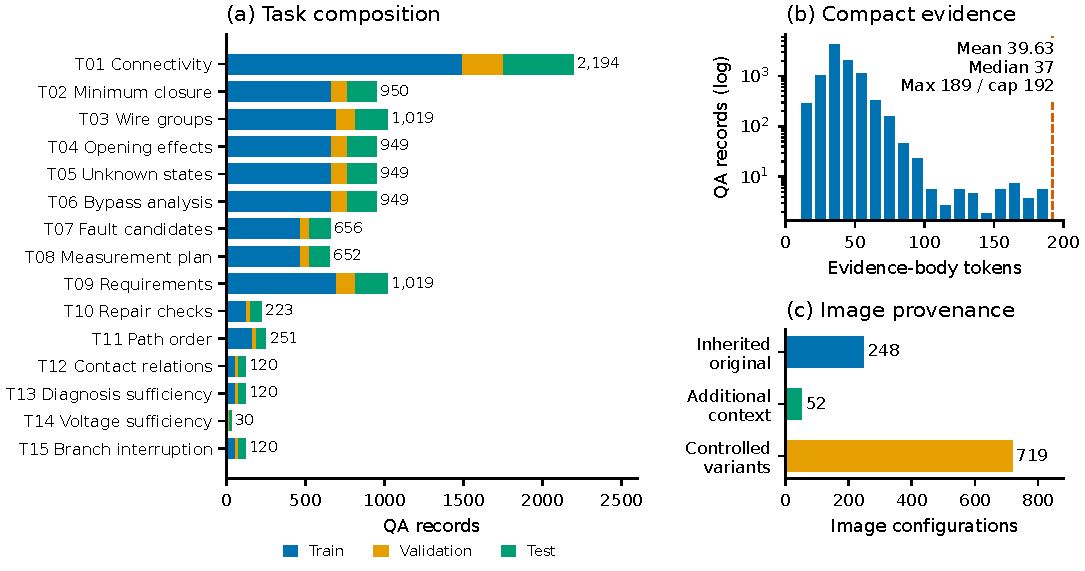
\includegraphics[width=\textwidth]{assets/figure_04.pdf}
\caption{Composition of the ELEC-VQA dataset: (a) QA by task and split; (b) evidence-body length under the local Qwen tokenizer, with logarithmic count scale and a 192-token cap; and (c) image provenance. Original windows may overlap within a drawing; controlled variants retain their parent-window identities.}
\label{fig:distribution}
\end{figure*}

\subsection{Interventions, Verification, and Partitions}
The 719 controlled variants include omitted wires, contact bypasses, wrong rewirings, and cross-network links. They are synthetic edits, not observed field-fault frequencies. Tasks are instantiated under explicit contact-state assignments and fault assumptions, with candidate questions retained only when their reference outcomes and evidence satisfy the corresponding verification queries.

The release audit replays 50,630 graph queries and checks training-view alignment, semantic-specification duplicates, file hashes, and split membership. The duplicate test compares task parameters and verification conditions within an image/task; it does not establish complete conceptual novelty or graph-isomorphism independence. Source rendering audits additionally check image decoding and geometry consistency. These checks establish consistency with the extracted representation, not independent expert correctness. A shared extraction error can survive graph replay.

Training, validation, and test contain 6,972, 1,155, and 2,074 QA over 697, 122, and 200 images, respectively. All source projects, DWGs, and parent families are disjoint across splits. Overlapping context windows and related variants remain grouped, but electrically similar templates may occur in different projects. Reporting follows the principle that composition, provenance, and reuse conditions should be documented explicitly~\cite{gebru2021datasheets}. The construction audit and independent reference-quality assessment are distinguished in Section~\ref{sec:experiments}.
